\section{Análisis exploratorio del DataSet}
El análisis exploratorio tiene como objetivo identificar el comportamiento de los datos a través del análisis estadístico. En este análisis se pueden visualizar en gran variaedad de tablas y gráficos que permitirán explorar las distribución de los datos e identificar comportamientos y/o características de las observaciones tales como; valores atípicos o outliers, concentraciones de valores, saltos o discontinuidades, forma de la distribución, etc.   



\subsection{Analisis inicial}
Lo primero que se va analizar es el comportamiento que tienen los datos en los diferentes años en las variables Total Población (TP), Total de Población no Hispana (TPNH) y Total de Población Hispana (TPH); donde se obtiene los siguientes resultados:
%\vspace{1mm}
\begin{kframe}
\begin{alltt}
        \hlstd{dfull} \hlkwb{<-} \hlkwd{data.frame}\hlstd{(}\hlkwc{TP}\hlstd{=datosnew}\hlopt{$}\hlstd{TP,}\hlkwc{TPNH}\hlstd{=datosnew}\hlopt{$}\hlstd{TPNH,}\hlkwc{TPH}\hlstd{=datosnew}\hlopt{$}\hlstd{TPH)}
        \hlkwd{stargazer}\hlstd{(dfull,}\hlkwc{type}\hlstd{=}\hlstr{"latex"}\hlstd{,}\hlkwc{title}\hlstd{=}\hlstr{"Total de la población de EEUU"}\hlstd{)}
\end{alltt}
\end{kframe}
% Table created by stargazer v.5.2 by Marek Hlavac, Harvard University. E-mail: hlavac at fas.harvard.edu
% Date and time: mar, abr 12, 2016 - 01:33:53 a.m.
\begin{table}[!htbp] \centering 
  \caption{Total de la población de EEUU} 
  \label{} 
\begin{tabular}{@{\extracolsep{5pt}}lccccc} 
\\[-1.8ex]\hline 
\hline \\[-1.8ex] 
Statistic & \multicolumn{1}{c}{N} & \multicolumn{1}{c}{Mean} & \multicolumn{1}{c}{St. Dev.} & \multicolumn{1}{c}{Min} & \multicolumn{1}{c}{Max} \\ 
\hline \\[-1.8ex] 
TP & 12,544 & 91,700.930 & 297,470.800 & 67 & 9,889,056 \\ 
TPNH & 12,544 & 78,932.380 & 214,518.700 & 60 & 5,511,922 \\ 
TPH & 12,544 & 12,768.550 & 102,278.800 & 0 & 4,760,974 \\ 
\hline \\[-1.8ex] 
\end{tabular} 
\end{table} 


%\vspace{1mm}
Es importane recordar que el anális principal de esta investigación se enfoca en estimar el crecimiento de la población hispana en las ciudades de EEUU, y revisando los resultados anteriores de la variable TPH se evidencia una media muy baja y es un valor muy insignificativo teniendo encuenta los valores de máximo y mínimo de la misma.  Por tal razón se ha hace necesario visaualizar a través de un gráfico mejor los datos de la variable TPH.   

\begin{figure}[H]
	\centering
\begin{knitrout}
\definecolor{shadecolor}{rgb}{0.969, 0.969, 0.969}\color{fgcolor}\begin{kframe}
\begin{alltt}
        \hlkwd{ggplot}\hlstd{(datosnew,}\hlkwd{aes}\hlstd{(TPH),}\hlkwd{label}\hlstd{(}\hlstr{""}\hlstd{))} \hlopt{+} \hlkwd{geom_dotplot}\hlstd{()}
\end{alltt}
\end{kframe}
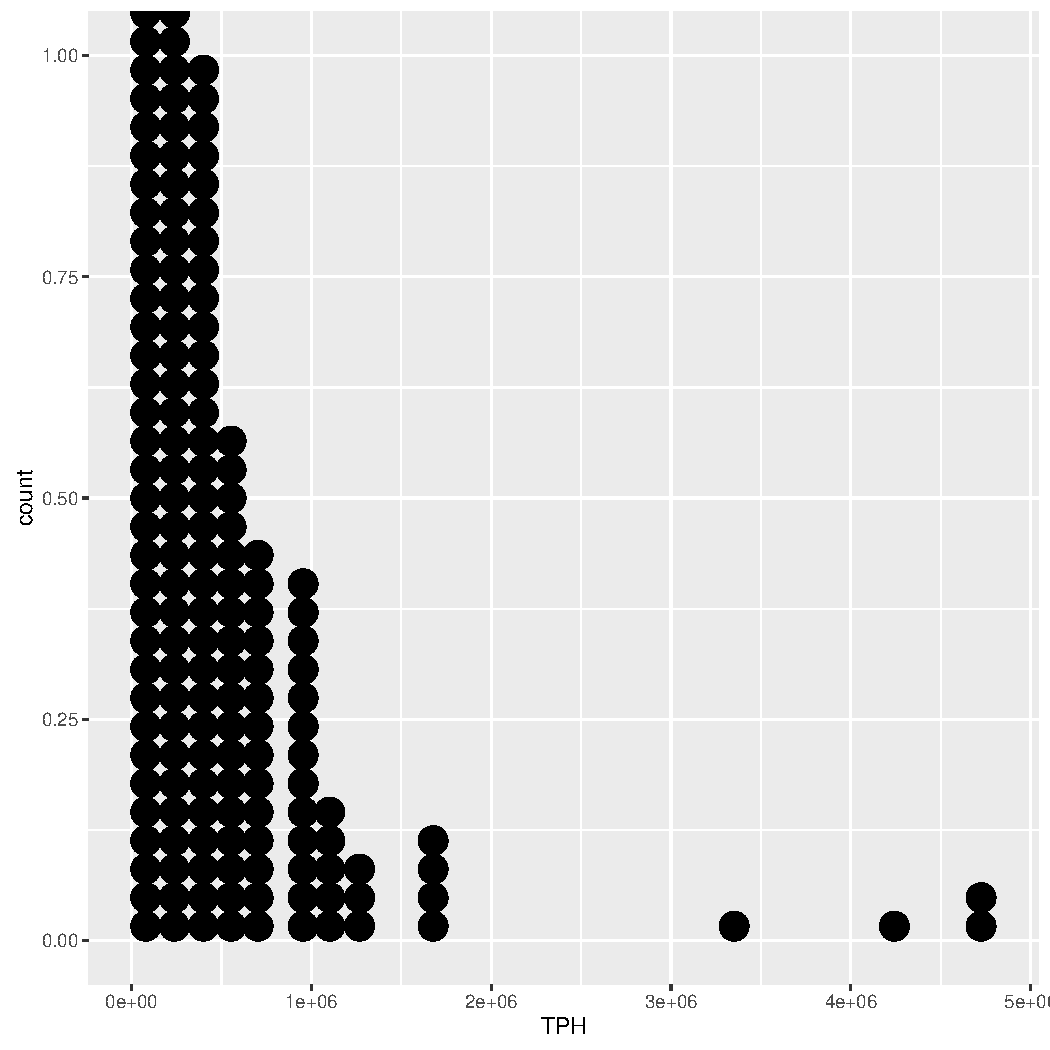
\includegraphics[width=\maxwidth]{figure/atipicos-1} 

\end{knitrout}
	\caption{Dotplot de la variable TPH}
\end{figure}


Posteriormente se procede a realizar un análisis del conjunto de datos más al detalle, de acuerdo con la información que se tiene de los diferentes años de la muestra.

%\vspace{-10mm}
\subsection{Analizando población hispana en el año 1990}
%Los datos más representativos se dan a continuación:
\begin{kframe}
\begin{alltt}
        \hlstd{d1990} \hlkwb{<-} \hlkwd{data.frame}\hlstd{(}\hlkwc{TotalCiudadanos}\hlstd{=datos1990}\hlopt{$}\hlstd{TP,}\hlkwc{TotalNoHispanos}\hlstd{=datos1990}\hlopt{$}\hlstd{TPNH,}\hlkwc{TotalHispanos}\hlstd{=datos1990}\hlopt{$}\hlstd{TPH)}
        \hlkwd{stargazer}\hlstd{(d1990,}\hlkwc{type}\hlstd{=}\hlstr{"latex"}\hlstd{,}\hlkwc{title}\hlstd{=}\hlstr{"Total de la población de EEUU en el año 1990"}\hlstd{)}
\end{alltt}
\end{kframe}
% Table created by stargazer v.5.2 by Marek Hlavac, Harvard University. E-mail: hlavac at fas.harvard.edu
% Date and time: mar, abr 12, 2016 - 01:33:54 a.m.
\begin{table}[!htbp] \centering 
  \caption{Total de la población de EEUU en el año 1990} 
  \label{} 
\begin{tabular}{@{\extracolsep{5pt}}lccccc} 
\\[-1.8ex]\hline 
\hline \\[-1.8ex] 
Statistic & \multicolumn{1}{c}{N} & \multicolumn{1}{c}{Mean} & \multicolumn{1}{c}{St. Dev.} & \multicolumn{1}{c}{Min} & \multicolumn{1}{c}{Max} \\ 
\hline \\[-1.8ex] 
TotalCiudadanos & 3,136 & 79,300.610 & 264,006.100 & 107 & 8,863,164 \\ 
TotalNoHispanos & 3,136 & 72,172.490 & 208,127.900 & 93 & 5,511,922 \\ 
TotalHispanos & 3,136 & 7,128.126 & 71,748.130 & 0 & 3,351,242 \\ 
\hline \\[-1.8ex] 
\end{tabular} 
\end{table} 


%\vspace{-10mm}
\begin{figure}[H]
	\centering
\begin{knitrout}
\definecolor{shadecolor}{rgb}{0.969, 0.969, 0.969}\color{fgcolor}\begin{kframe}
\begin{alltt}
        \hlkwd{ggplot}\hlstd{(datos1990,}\hlkwd{aes}\hlstd{(TPH))} \hlopt{+} \hlkwd{geom_histogram}\hlstd{()}
\end{alltt}
\end{kframe}
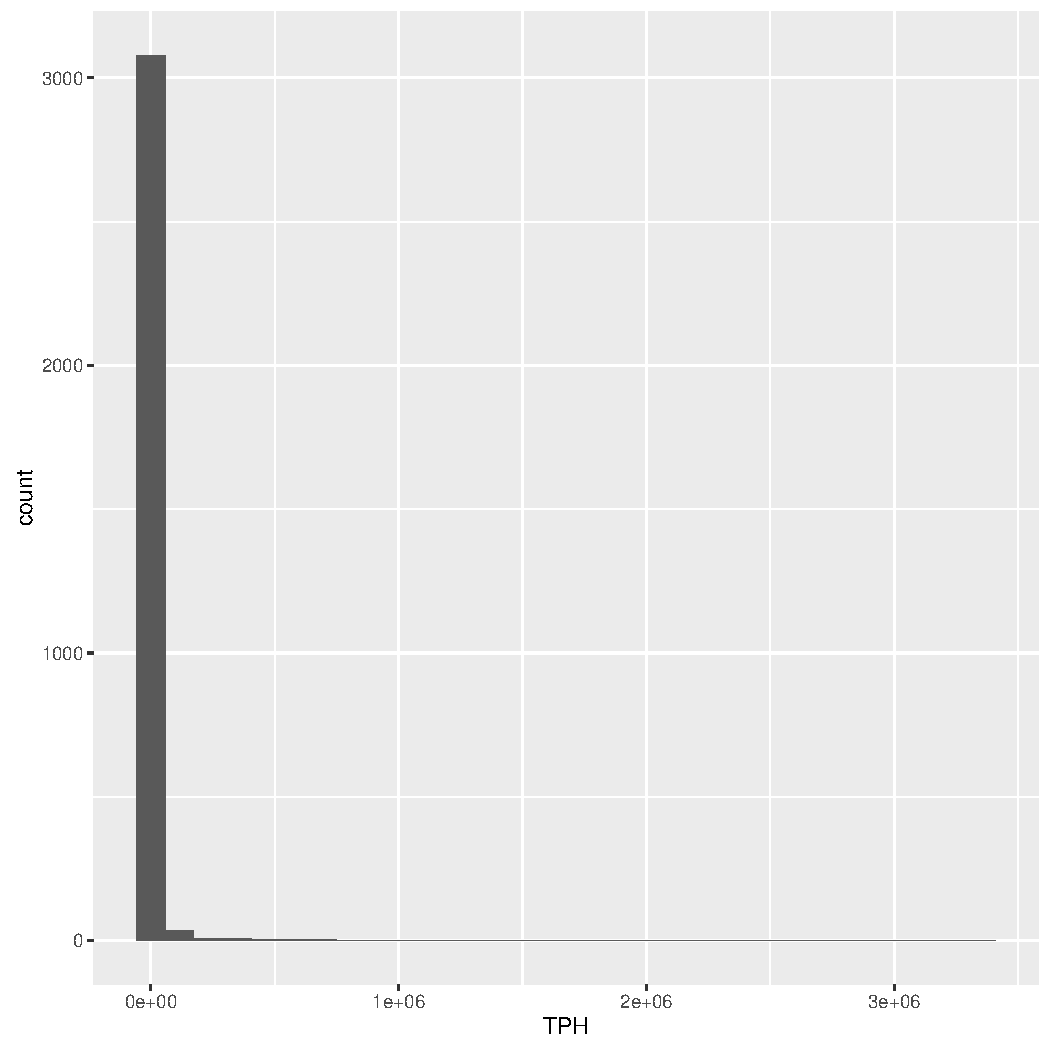
\includegraphics[width=\maxwidth]{figure/pobHis1990-1} 

\end{knitrout}
	\caption{Población Hispana en el año 1990}
\end{figure}

%\vspace{-10mm}
\subsection{Analizando población hispana en el año 2000}
%Los datos más representativos se dan a continuación:
\begin{kframe}
\begin{alltt}
        \hlstd{d2000} \hlkwb{<-} \hlkwd{data.frame}\hlstd{(}\hlkwc{TotalCiudadanos}\hlstd{=datos2000}\hlopt{$}\hlstd{TP,}\hlkwc{TotalNoHispanos}\hlstd{=datos2000}\hlopt{$}\hlstd{TPNH,}\hlkwc{TotalHispanos}\hlstd{=datos2000}\hlopt{$}\hlstd{TPH)}
        \hlkwd{stargazer}\hlstd{(d2000,}\hlkwc{type}\hlstd{=}\hlstr{"latex"}\hlstd{,}\hlkwc{title}\hlstd{=}\hlstr{"Total de la población de EEUU en el año 2000"}\hlstd{)}
\end{alltt}
\end{kframe}
% Table created by stargazer v.5.2 by Marek Hlavac, Harvard University. E-mail: hlavac at fas.harvard.edu
% Date and time: mar, abr 12, 2016 - 01:33:54 a.m.
\begin{table}[!htbp] \centering 
  \caption{Total de la población de EEUU en el año 2000} 
  \label{} 
\begin{tabular}{@{\extracolsep{5pt}}lccccc} 
\\[-1.8ex]\hline 
\hline \\[-1.8ex] 
Statistic & \multicolumn{1}{c}{N} & \multicolumn{1}{c}{Mean} & \multicolumn{1}{c}{St. Dev.} & \multicolumn{1}{c}{Min} & \multicolumn{1}{c}{Max} \\ 
\hline \\[-1.8ex] 
TotalCiudadanos & 3,136 & 89,735.040 & 292,674.700 & 67 & 9,519,338 \\ 
TotalNoHispanos & 3,136 & 78,476.900 & 214,891.300 & 60 & 5,277,125 \\ 
TotalHispanos & 3,136 & 11,258.140 & 96,312.440 & 1 & 4,242,213 \\ 
\hline \\[-1.8ex] 
\end{tabular} 
\end{table} 


%\vspace{-5mm}
\begin{figure}[H]
	\centering
\begin{knitrout}
\definecolor{shadecolor}{rgb}{0.969, 0.969, 0.969}\color{fgcolor}\begin{kframe}
\begin{alltt}
        \hlkwd{ggplot}\hlstd{(datos2000,}\hlkwd{aes}\hlstd{(TPH))} \hlopt{+} \hlkwd{geom_histogram}\hlstd{()}
\end{alltt}
\end{kframe}
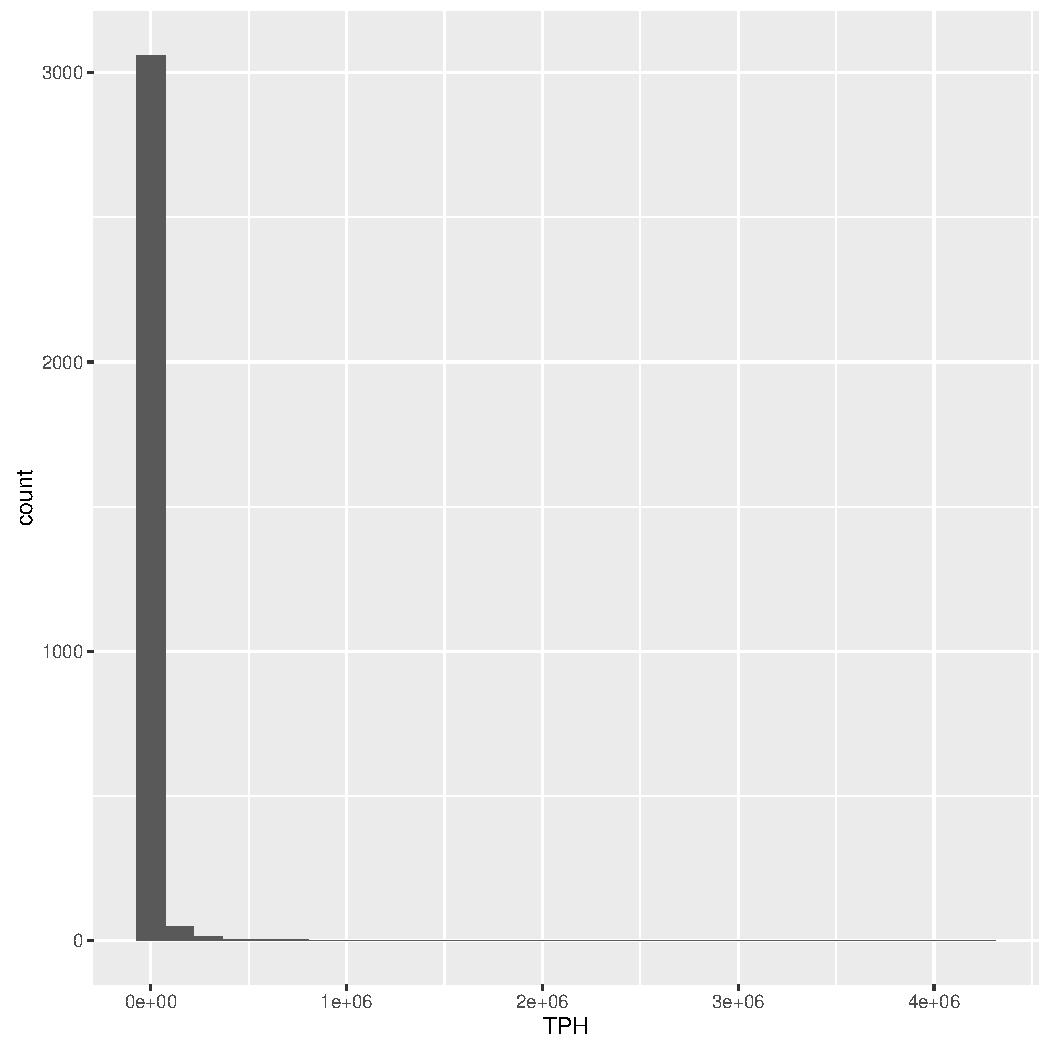
\includegraphics[width=\maxwidth]{figure/pobHisp2000-1} 

\end{knitrout}
	\caption{Población Hispana en el año 2000}
\end{figure}

%\vspace{-10mm}
\subsection{Analizando población hispana en el año 2010}
%Los datos más representativos se dan a continuación:
\begin{kframe}
\begin{alltt}
        \hlstd{d2010} \hlkwb{<-} \hlkwd{data.frame}\hlstd{(}\hlkwc{TotalCiudadanos}\hlstd{=datos2010}\hlopt{$}\hlstd{TP,}\hlkwc{TotalNoHispanos}\hlstd{=datos2010}\hlopt{$}\hlstd{TPNH,}\hlkwc{TotalHispanos}\hlstd{=datos2010}\hlopt{$}\hlstd{TPH)}
        \hlkwd{stargazer}\hlstd{(d2010,}\hlkwc{type}\hlstd{=}\hlstr{"latex"}\hlstd{,}\hlkwc{title}\hlstd{=}\hlstr{"Total de la población de EEUU en el año 2010"}\hlstd{)}
\end{alltt}
\end{kframe}
% Table created by stargazer v.5.2 by Marek Hlavac, Harvard University. E-mail: hlavac at fas.harvard.edu
% Date and time: mar, abr 12, 2016 - 01:33:54 a.m.
\begin{table}[!htbp] \centering 
  \caption{Total de la población de EEUU en el año 2010} 
  \label{} 
\begin{tabular}{@{\extracolsep{5pt}}lccccc} 
\\[-1.8ex]\hline 
\hline \\[-1.8ex] 
Statistic & \multicolumn{1}{c}{N} & \multicolumn{1}{c}{Mean} & \multicolumn{1}{c}{St. Dev.} & \multicolumn{1}{c}{Min} & \multicolumn{1}{c}{Max} \\ 
\hline \\[-1.8ex] 
TotalCiudadanos & 3,136 & 98,430.440 & 313,221.000 & 82 & 9,818,605 \\ 
TotalNoHispanos & 3,136 & 82,336.350 & 216,856.000 & 64 & 5,130,716 \\ 
TotalHispanos & 3,136 & 16,094.090 & 115,731.900 & 0 & 4,687,889 \\ 
\hline \\[-1.8ex] 
\end{tabular} 
\end{table} 


%\vspace{-5mm}
\begin{figure}[H]
	\centering
\begin{knitrout}
\definecolor{shadecolor}{rgb}{0.969, 0.969, 0.969}\color{fgcolor}\begin{kframe}
\begin{alltt}
        \hlkwd{ggplot}\hlstd{(datos2010,}\hlkwd{aes}\hlstd{(TPH))} \hlopt{+} \hlkwd{geom_histogram}\hlstd{()}
\end{alltt}
\end{kframe}
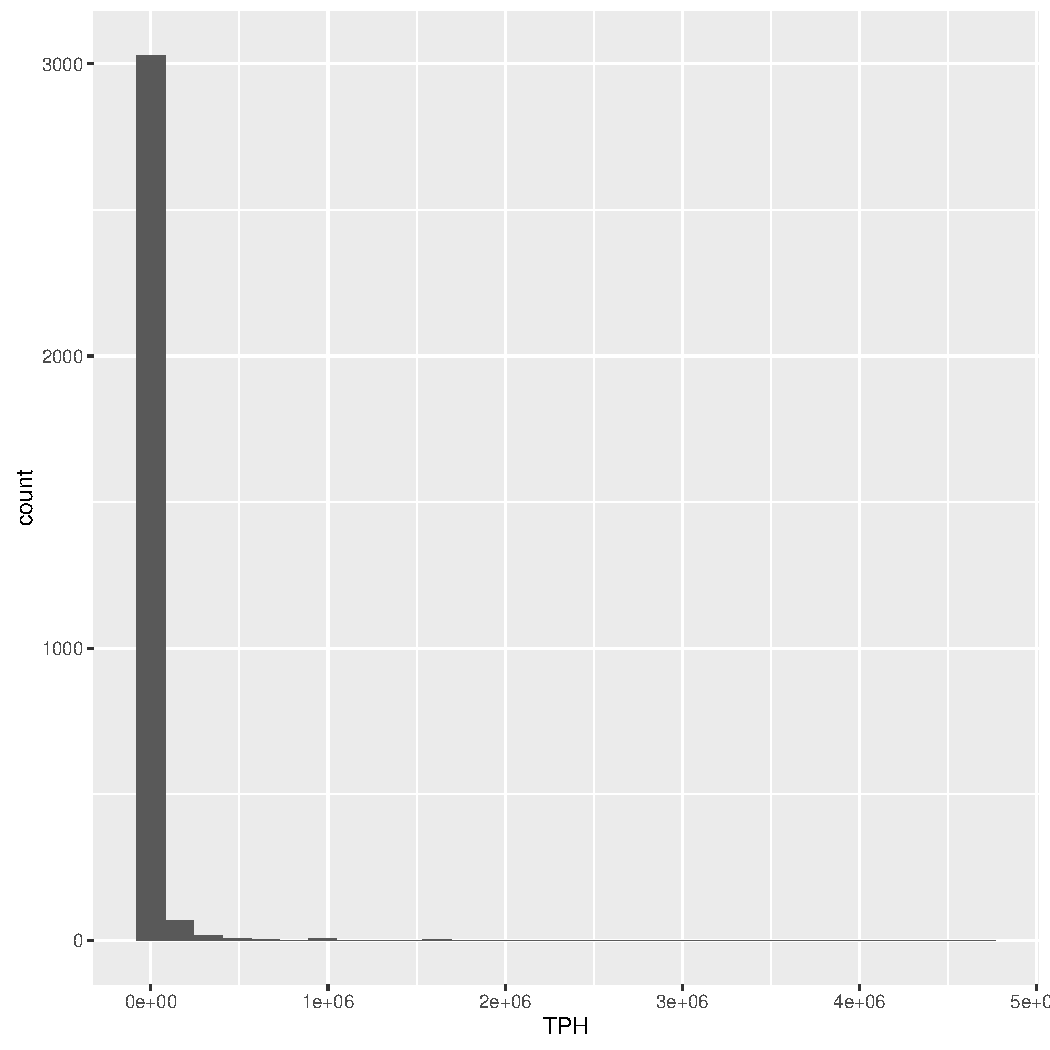
\includegraphics[width=\maxwidth]{figure/pobHisp2010-1} 

\end{knitrout}
	\caption{Población Hispana en el año 2010}
\end{figure}

%\vspace{-10mm}
\subsection{Analizando población hispana en el año 2011}
%Los datos más representativos se dan a continuación:
\begin{kframe}
\begin{alltt}
        \hlstd{d2011} \hlkwb{<-} \hlkwd{data.frame}\hlstd{(}\hlkwc{TotalCiudadanos}\hlstd{=datos2011}\hlopt{$}\hlstd{TP,}\hlkwc{TotalNoHispanos}\hlstd{=datos2011}\hlopt{$}\hlstd{TPNH,}\hlkwc{TotalHispanos}\hlstd{=datos2011}\hlopt{$}\hlstd{TPH)}
        \hlkwd{stargazer}\hlstd{(d2011,}\hlkwc{type}\hlstd{=}\hlstr{"latex"}\hlstd{,}\hlkwc{title}\hlstd{=}\hlstr{"Total de la población de EEUU en el año 2011"}\hlstd{)}
\end{alltt}
\end{kframe}
% Table created by stargazer v.5.2 by Marek Hlavac, Harvard University. E-mail: hlavac at fas.harvard.edu
% Date and time: mar, abr 12, 2016 - 01:33:55 a.m.
\begin{table}[!htbp] \centering 
  \caption{Total de la población de EEUU en el año 2011} 
  \label{} 
\begin{tabular}{@{\extracolsep{5pt}}lccccc} 
\\[-1.8ex]\hline 
\hline \\[-1.8ex] 
Statistic & \multicolumn{1}{c}{N} & \multicolumn{1}{c}{Mean} & \multicolumn{1}{c}{St. Dev.} & \multicolumn{1}{c}{Min} & \multicolumn{1}{c}{Max} \\ 
\hline \\[-1.8ex] 
TotalCiudadanos & 3,136 & 99,337.630 & 316,723.400 & 90 & 9,889,056 \\ 
TotalNoHispanos & 3,136 & 82,743.800 & 217,998.000 & 76 & 5,128,082 \\ 
TotalHispanos & 3,136 & 16,593.830 & 118,221.400 & 0 & 4,760,974 \\ 
\hline \\[-1.8ex] 
\end{tabular} 
\end{table} 


%\vspace{-10mm}
\begin{figure}[H]
	\centering
\begin{knitrout}
\definecolor{shadecolor}{rgb}{0.969, 0.969, 0.969}\color{fgcolor}\begin{kframe}
\begin{alltt}
        \hlkwd{ggplot}\hlstd{(datos2011,}\hlkwd{aes}\hlstd{(TPH))} \hlopt{+} \hlkwd{geom_histogram}\hlstd{()}
\end{alltt}
\end{kframe}
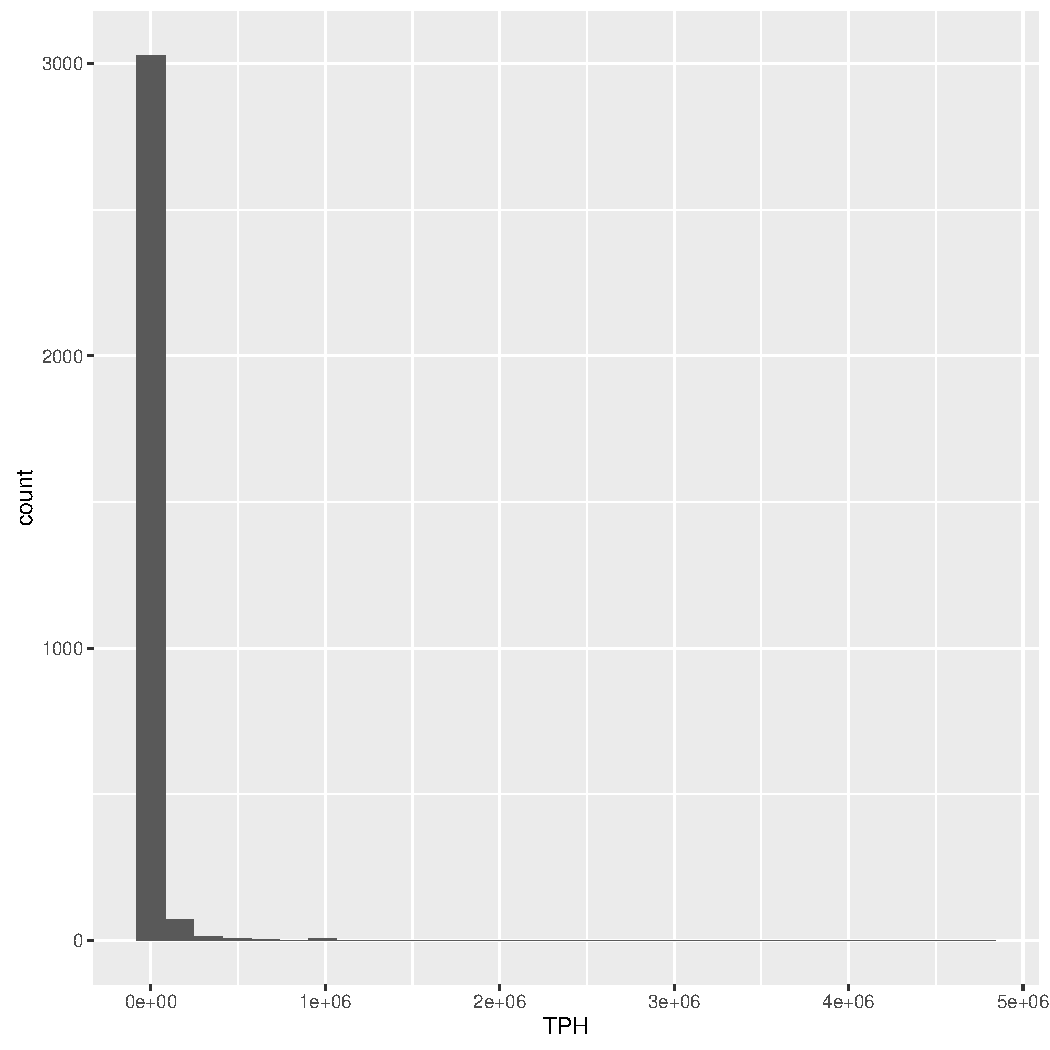
\includegraphics[width=\maxwidth]{figure/pobHisp2011-1} 

\end{knitrout}
	\caption{Población Hispana en el año 2011}
\end{figure}

%\vspace{-10mm}
\subsection{Percentiles del conjunto de datos}
El percentil de orden \(k\) es el cuantil de orden \(\dfrac {k} {100}\). El recorrido intercuantil refleja la variabilidad de las observaciones comprendidas entre los percentiles 25 y 75 en el conjunto de datos. En esta sesión se obtienen los percentiles del 25\%,  50\% y 75\% de las variables Total Población (TP) y Total Población Hispana (TPH) en los diferentes años de la muestra.

%\vspace{4mm}
%\begin{itemize}
%\item Percentiles del población en el año 1990
% latex table generated in R 3.2.3 by xtable 1.8-2 package
% Tue Apr 12 01:33:55 2016
\begin{table}[ht]
\centering
\begin{tabular}{rrrr}
  \hline
 & PercentilesTP & PercentilesTPH & PercentilesTPNH \\ 
  \hline
25\% & 10360.00 & 67.00 & 9836.75 \\ 
  50\% & 22224.00 & 208.00 & 21362.00 \\ 
  75\% & 54771.50 & 1159.00 & 53324.00 \\ 
   \hline
\end{tabular}
\caption{Percentiles de TP, TPH y TPNH en el año 1990} 
\end{table}


% latex table generated in R 3.2.3 by xtable 1.8-2 package
% Tue Apr 12 01:33:55 2016
\begin{table}[ht]
\centering
\begin{tabular}{rrrr}
  \hline
 & PercentilesTP & PercentilesTPH & PercentilesTPNH \\ 
  \hline
25\% & 11264.25 & 155.00 & 10431.50 \\ 
  50\% & 24658.00 & 493.00 & 23244.00 \\ 
  75\% & 61844.25 & 2411.50 & 58906.00 \\ 
   \hline
\end{tabular}
\caption{Percentiles de TP, TPH y TPNH en el año 2000} 
\end{table}

	
% latex table generated in R 3.2.3 by xtable 1.8-2 package
% Tue Apr 12 01:33:55 2016
\begin{table}[ht]
\centering
\begin{tabular}{rrrr}
  \hline
 & PercentilesTP & PercentilesTPH & PercentilesTPNH \\ 
  \hline
25\% & 11154.75 & 262.75 & 10154.25 \\ 
  50\% & 25901.50 & 892.00 & 24016.00 \\ 
  75\% & 67012.50 & 4226.25 & 62438.50 \\ 
   \hline
\end{tabular}
\caption{Percentiles de TP, TPH y TPNH en el año 2010} 
\end{table}

	
% latex table generated in R 3.2.3 by xtable 1.8-2 package
% Tue Apr 12 01:33:55 2016
\begin{table}[ht]
\centering
\begin{tabular}{rrrr}
  \hline
 & PercentilesTP & PercentilesTPH & PercentilesTPNH \\ 
  \hline
25\% & 11145.00 & 284.00 & 10125.75 \\ 
  50\% & 25896.00 & 926.00 & 23962.00 \\ 
  75\% & 67398.75 & 4417.75 & 62925.75 \\ 
   \hline
\end{tabular}
\caption{Percentiles de TP, TPH y TPNH en el año 2011} 
\end{table}

